\chapter{Simulation methods}\label{chap5}

In the previous chapters, we focused on conjugate families, where the posterior and predictive distributions have standard analytical forms (e.g., normal, Student's t, gamma, binomial, Poisson, etc.) and where the marginal likelihood has a closed-form analytical solution. However, realistic models are often more complex and lack such closed-form solutions.

To address this complexity, we rely on simulation (stochastic) methods to draw samples from posterior and predictive distributions. This chapter introduces posterior simulation, a cornerstone of Bayesian inference. We discuss Markov Chain Monte Carlo (MCMC) methods, including Gibbs sampling, Metropolis-Hastings, and Hamiltonian Monte Carlo, as well as other techniques like importance sampling and sequential Monte Carlo.

The simulation methods discussed in this chapter are specifically applied throughout this book. However, we do not delve into deterministic methods, such as numerical integration (quadrature), or other simulation methods, including discrete approximation, the probability integral transform, the method of composition, accept-reject sampling, and slice sampling algorithms. While these methods are also widely used, they are not as common as the approaches explicitly employed in this book.

For readers interested in these alternative methods, we recommend exploring \cite[Chaps.~2 and 3]{robert2010introducing}, \cite[Chaps.~2, 3, and 8]{robert2011monte}, \cite[Chap.~5]{greenberg2012introduction}, and \cite[Chap.~10]{gelman2021bayesian}.

%\section{The inverse transform method}\label{sec51}

%\section{Method of composition}\label{sec52}

%\section{Accept and reject algorithm}\label{sec53}

\section{Markov chain Monte Carlo methods}\label{sec51}

Markov Chain Monte Carlo (MCMC) methods are algorithms used to approximate complex probability distributions by constructing a Markov chain. This chain is a sequence of random samples where each sample depends only on the previous one. The goal of MCMC methods is to obtain draws from the posterior distribution as the equilibrium distribution. The key point in MCMC methods is the transition kernel or density, $\pi(\bm{\theta}^{(s)}|\bm{\theta}^{(s-1)})$, which generates a draw $\bm{\theta}^{(s)}$ at stage $s$ that depends solely on $\bm{\theta}^{(s-1)}$. This transition distribution must be designed such that the Markov chain converges to a unique stationary distribution, which, in our case, is the posterior distribution, that is, $\pi(\bm{\theta}^{(s)}|\bm{y})=\int_{\bm{\Theta}}\pi(\bm{\theta}^{(s)}|\bm{\theta}^{(s-1)},\bm{y})\pi(\bm{\theta}^{(s-1)}|\bm{y})d\bm{\theta}^{(s-1)}$.

Given that we start at an arbitrary point, $\bm{\theta}^{(0)}$, the algorithm requires that the Markov chain be \textit{irreducible}, meaning that the process can reach any other state with positive probability. Additionally, the process must be \textit{aperiodic}, meaning that for each state, the greatest common divisor of the number of steps it takes to return to the state is 1, ensuring that there are no cycles forcing the system to return to a state only after a fixed number of steps. Furthermore, the process must be \textit{recurrent}, meaning that it will return to any state an infinite number of times with probability one. However, to ensure convergence to the stationary distribution, a stronger condition is required: the process must be \textit{positive recurrent}, meaning that the expected return time to a state is finite. Given an \textit{irreducible}, \textit{aperiodic}, and \textit{positive recurrent} transition density, the Markov chain algorithm will asymptotically converge to the stationary posterior distribution we are seeking. For more details, see \cite[chap.~6]{robert2011monte}.
   

%\subsection{Some theory}\label{sec551}

\subsection{Gibbs sampler}\label{sec511}

This Gibbs sampler algorithm is one of the most widely used MCMC methods for sampling from non-standard distributions in Bayesian analysis. While it is a special case of the Metropolis-Hastings (MH) algorithm, it originated from a different theoretical background \cite{Geman1984}. The key requirement for implementing the Gibbs sampling algorithm is the availability of conditional posterior distributions. The algorithm works by cycling through the conditional posterior distributions corresponding to different blocks of the parameter space under inference.

Two simplify concepts let's focus on a parameter space composed by two blocks, $\bm{\theta} = [\bm{\theta}_1 \ \bm{\theta}_2]^{\top}$, the Gibbs sampling algorithm uses as transition kernel $\pi(\bm{\theta}_1^{(s)},\bm{\theta}_2^{(s)}|\bm{\theta}_1^{(s-1)},\bm{\theta}_2^{(s-1)},\bm{y})=\pi(\bm{\theta}_1^{(s)}|\bm{\theta}_2^{(s-1)},\bm{y})\pi(\bm{\theta}_2^{(s)}|\bm{\theta}_1^{(s)},\bm{y})$. Thus,
{\scriptsize
\begin{align*}
	\int_{\bm{\Theta}}\pi(\bm{\theta}^{(s)}|\bm{\theta}^{(s-1)},\bm{y})\pi(\bm{\theta}^{(s-1)}|\bm{y})d\bm{\theta}^{(s-1)}
	&=\int_{\bm{\Theta}_2}\int_{\bm{\Theta}_1}\pi(\bm{\theta}_1^{(s)}|\bm{\theta}_2^{(s-1)},\bm{y})\pi(\bm{\theta}_2^{(s)}|\bm{\theta}_1^{(s)},\bm{y})\pi(\bm{\theta}^{(s-1)}_1,\bm{\theta}^{(s-1)}_2|\bm{y})d\bm{\theta}^{(s-1)}_1d\bm{\theta}^{(s-1)}_2\\
	&=\pi(\bm{\theta}_2^{(s)}|\bm{\theta}_1^{(s)},\bm{y})\int_{\bm{\Theta}_2}\int_{\bm{\Theta}_1}\pi(\bm{\theta}_1^{(s)}|\bm{\theta}_2^{(s-1)},\bm{y})\pi(\bm{\theta}^{(s-1)}_1,\bm{\theta}^{(s-1)}_2|\bm{y})d\bm{\theta}^{(s-1)}_1d\bm{\theta}^{(s-1)}_2\\
	&=\pi(\bm{\theta}_2^{(s)}|\bm{\theta}_1^{(s)},\bm{y})\int_{\bm{\Theta}_2}\pi(\bm{\theta}_1^{(s)}|\bm{\theta}_2^{(s-1)},\bm{y})\pi(\bm{\theta}^{(s-1)}_2|\bm{y})d\bm{\theta}^{(s-1)}_2\\
	&=\pi(\bm{\theta}_2^{(s)}|\bm{\theta}_1^{(s)},\bm{y})\int_{\bm{\Theta}_2}\pi(\bm{\theta}_1^{(s)},\bm{\theta}_2^{(s-1)}|\bm{y})d\bm{\theta}^{(s-1)}_2\\
	&=\pi(\bm{\theta}_2^{(s)}|\bm{\theta}_1^{(s)},\bm{y})\pi(\bm{\theta}_1^{(s)}|\bm{y})\\
	&=\pi(\bm{\theta}_1^{(s)},\bm{\theta}_2^{(s)}|\bm{y}).\\
\end{align*}
}
Then, $\pi(\bm{\theta}|\bm{y})$ is the stationary distribution for the Gibbs transition kernel.

A word of caution! Even if we have well-defined conditional posterior distributions $\pi(\bm{\theta}_1^{(s)} \mid \bm{\theta}_2^{(s-1)}, \bm{y})$ and $\pi(\bm{\theta}_2^{(s)} \mid \bm{\theta}_1^{(s)}, \bm{y})$, and we can simulate from them, the joint posterior distribution $\pi(\bm{\theta}_1^{(s)}, \bm{\theta}_2^{(s)} \mid \bm{y})$ may not correspond to any proper distribution. We should be mindful of this situation, especially when dealing with improper prior distributions (see \cite[Chap.~10]{robert2011monte} for details).

Algorithm \ref{Alg:Gibbs} shows how to implement a Gibbs sampler with $d$ blocks. 

\begin{algorithm}[h!]
	\caption{Gibbs sampling}\label{Alg:Gibbs}
	\begin{algorithmic}[1]  		 			
		\State Set $\bm{\theta}_2^{(0)}$, $\bm{\theta}_3^{(0)}$, ..., $\bm{\theta}_d^{(0)}$
		\For{\texttt{$s=1,\dots,S$}}
		\State Draw $\bm{\theta}_1^{(s)}$ from $\pi(\bm{\theta}_1^{(s)}|\bm{\theta}_2^{(s-1)},\dots,\bm{\theta}_d^{(s-1)})$
		\State Draw $\bm{\theta}_2^{(s)}$ from $\pi(\bm{\theta}_2^{(s)}|\bm{\theta}_1^{(s)},\dots,\bm{\theta}_d^{(s-1)})$
		\State $\vdots$
		\State Draw $\bm{\theta}_d^{(s)}$ from $\pi(\bm{\theta}_d^{(s)}|\bm{\theta}_2^{(s)},\dots,\bm{\theta}_{d-1}^{(s)})$ 
		\EndFor 
		\end{algorithmic} 
\end{algorithm}

\textbf{Example: The normal model with independent priors}

Let's recap the math test exercise in Chapter \ref{chap4}, this time assuming independent priors. Specifically, let $Y_i \sim N(\mu, \sigma^2)$, where $\mu \sim N(\mu_0, \sigma_0^2)$ and $\sigma^2 \sim IG(\alpha_0 / 2, \delta_0 / 2)$. The sample size is 50, and the mean and standard deviation of the math scores are 102 and 10, respectively. We set $\mu_0 = 100$, $\sigma_0^2 = 100$, and $\alpha_0 = \delta_0 = 0.001$.

The posterior distribution is
\begin{align*}
	\pi(\mu,\sigma^2|\bm{y})&\propto (\sigma^2)^{-N/2}\exp\left\{-\frac{1}{2\sigma^2}\sum_{i=1}^N(y_i-\mu)^2\right\}\\
	&\times \exp\left\{-\frac{1}{2\sigma^2_0}(\mu-\mu_0)^2\right\}\times \left(\frac{1}{\sigma^2}\right)^{\alpha_0/2+1}\exp\left\{-\frac{\delta_0}{2\sigma^2}\right\}.
\end{align*}
Thus, the conditional posterior distribution of $\mu$ is
\begin{align*}
	\pi(\mu,\sigma^2|\bm{y})&\propto \exp\left\{-\frac{1}{2}\left[\frac{1}{\sigma^2}\sum_{i=1}^N(y_i-\mu)^2+\frac{1}{\sigma^2_0}(\mu-\mu_0)^2\right]\right\}\\
	&\propto \exp\left\{-\frac{1}{2}\left[\mu^2\left(\frac{1}{\sigma^2/N}+\frac{1}{\sigma^2_0}\right)-2\mu\left(\frac{\bar{y}}{\sigma^2/N}+\frac{\mu_0}{\sigma_0^2}\right)\right]\right\}.  
\end{align*} 
We set $\mu_n=\sigma^{2}_n\left(\frac{\bar{y}}{\sigma^2/N}+\frac{\mu_0}{\sigma_0^2}\right)$ and $\sigma^{2}_n=\left(\frac{1}{\sigma^2/N}+\frac{1}{\sigma_0^2}\right)^{-1}$. Thus,
\begin{align*}
	\pi(\mu,\sigma^2|\bm{y})&\propto \exp\left\{-\frac{1}{2\sigma_n^2}\left[\mu^2-2\mu\mu_n+\mu_n^2-\mu_n^2\right]\right\}\\
	&\propto \exp\left\{-\frac{1}{2\sigma_n^2}(\mu-\mu_n)^2\right\}.\\  
\end{align*} 
This is the kernel of a normal distribution, that is, $\mu|\sigma^2,\bm{y}\sim N(\mu_n,\sigma_n^2)$.

The conditional posterior distribution of $\sigma^2$ is given by
\begin{align*}
	\pi(\sigma^2|\mu,\bm{y})&\propto (\sigma^2)^{-N/2}\exp\left\{-\frac{1}{2\sigma^2}\sum_{i=1}^N(y_i-\mu)^2\right\}\\
	&\times \left(\frac{1}{\sigma^2}\right)^{\alpha_0/2+1}\exp\left\{-\frac{\delta_0}{2\sigma^2}\right\}\\
	&\propto (\sigma^2)^{-N/2-\alpha_0/2-1} \exp\left\{-\frac{1}{2\sigma^2}\left[\sum_{i=1}^N(y_i-\mu)^2+\delta_0\right]\right\}.
\end{align*} 
Thus, $\sigma^2|\mu,\bm{y}\sim IG(\alpha_n/2,\delta_n/2)$, where $\alpha_n=N+\alpha_0$ and $\delta_n=\sum_{i=1}^N(y_i-\mu)^2+\delta_0=N\hat{\sigma}^2+N(\bar{y}-\mu)^2+\delta_0$ given that $\sum_{i=1}^N(y_i-\bar{y})=0$, where $\bar{y}$ and $\hat{\sigma}$ are the mean and standard deviation estimates.

As we have the conditional posterior distributions, we can use the Gibbs sampling algorithm to perform inference in this model. The following code shows how to do it.

\begin{tcolorbox}[enhanced,width=4.67in,center upper,
	fontupper=\large\bfseries,drop shadow southwest,sharp corners]
	\textit{R code. Gibbs sampler: The math example}
	\begin{VF}
		\begin{lstlisting}[language=R]
rm(list = ls()); set.seed(010101)
N <- 50 # Sample size
muhat <- 102 # Sample mean
sig2hat <- 100 # Sample variance
# Hyperparameters
mu0 <- 100; sig20 <- 100; delta0 <- 0.001; alpha0 <- 0.001
# MCMC parameters
MCMC <- 10000; burnin <- 1000; S <- MCMC + burnin
keep <- (burnin+1):S
# Posterior draws
sig2Post <- rep(NA, S)
muPost <- rep(NA, S)
alphan <- alpha0 + N; sig2 <- sig20
# Gibbs sampler
for(s in 1:S){
	sig2n <- (1/(sig2/N)+1/sig20)^(-1)
	mun <- sig2n*(muhat/(sig2/N)+mu0/sig20)
	mu <- rnorm(1, mun, sig2n^0.5)
	deltan <- N*(sig2hat + (muhat - mu)^2)
	sig2 <- invgamma::rinvgamma(1, shape = alphan, rate = deltan)
	muPost[s] <- mu;sig2Post[s] <- sig2
}
sig2s <- coda::mcmc(sig2Post[keep]) 
mus <- coda::mcmc(muPost[keep]) 
summary(sig2s); summary(mus)
hist(mus, main = "Histogram: Posterior mean", xlab = "Posterior mean", col = "blue", breaks = 50)
muPost_tq <- quantile(mus, c(0.025, 0.5, 0.975)); muPost_tq
PmuPost_tcutoff <- mean(mus > 102); PmuPost_tcutoff
\end{lstlisting}
	\end{VF}
\end{tcolorbox} 

\begin{figure}[!h]
	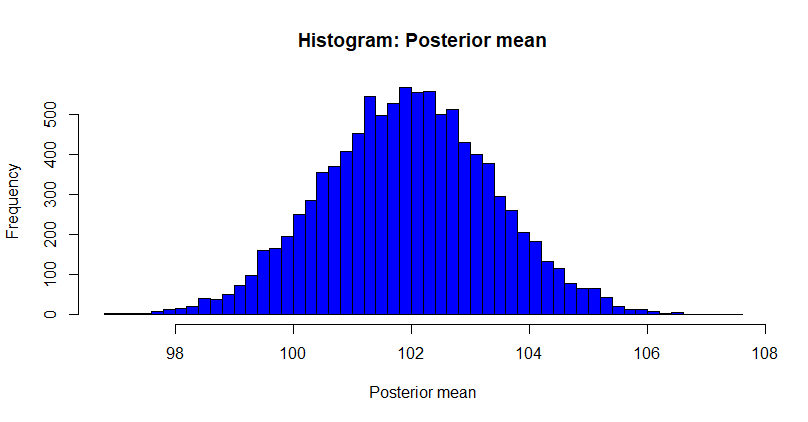
\includegraphics[width=340pt, height=200pt]{Chapters/chapter5/figures/PostMeanMathTest.png}
	%%\centerline{\epsfig{/Chapters/chapter1/figures/cat.eps,width=.8\textheight,height=.4\textwidth}}
	\caption[List of figure caption goes here]{Histogram of posterior draws of mean: Math test}\label{fig51}
\end{figure}

Figure \ref{fig51} shows the histogram of the draws of the posterior mean of the math test results. The posterior mean and median are 101.94 and 101.95, and the 95\% credible interval is (99.14, 104.79).\\


\textbf{Example: Mining disaster change point}

Let's use the dataset \textit{Mining.csv} provided by \cite{carlin1992hierarchical}.This dataset counts mining disasters per year from 1851 to 1962 in British coal mines. 

We assume that there is an unknown structural change point in the amount of mining disasters where the parameters of the Poisson distributions describing change. In particular,
\begin{align*}
	p(y_t)=\begin{Bmatrix}
		\frac{\exp(-\lambda_1)\lambda_1^{y_t}}{y_t!}, & t=1,2,\dots,H\\
		\frac{\exp(-\lambda_2)\lambda_2^{y_t}}{y_t!}, & t=H+1,\dots,T\\
	\end{Bmatrix},
\end{align*}  
where $H$ is the changing point.

We use conjugate families for $\lambda_l$, $l=1,2$, that is, $\lambda_l\sim G(\alpha_{l0},\delta_{l0})$, and set $\pi(H)=1/T$, that is, an discrete uniform distribution for the changing point. 

\textbf{Example: Linear regression electricity demand}
Let's recap the electricity demand example in Chapter \ref{chap4}.  

\textbf{Example: Multivariate normal model, utility demand}
Let's recap the utility demand exercise in Chapter \ref{chap4}. 



\subsection{Metropolis-Hastings}\label{sec512}

\section{Importance sampling}\label{sec52}

\section{Sequential Monte Carlo}\label{sec53}

\section{Hamiltonian Monte Carlo}\label{sec54}

\section{Convergence diagnostics}\label{sec55}
\subsection{Numerical standard error}
\subsection{Effective sample size}
\subsection{Checking for errors in the posterior simulator}
\cite{geweke2004getting}